\documentclass[11pt, oneside]{article} 
\usepackage{geometry}
\geometry{letterpaper} 
\usepackage{graphicx}
	
\usepackage{amssymb}
\usepackage{amsmath}
\usepackage{parskip}
\usepackage{color}
\usepackage{hyperref}

\graphicspath{{/Users/telliott_admin/Tex/png/}}
% \begin{center} 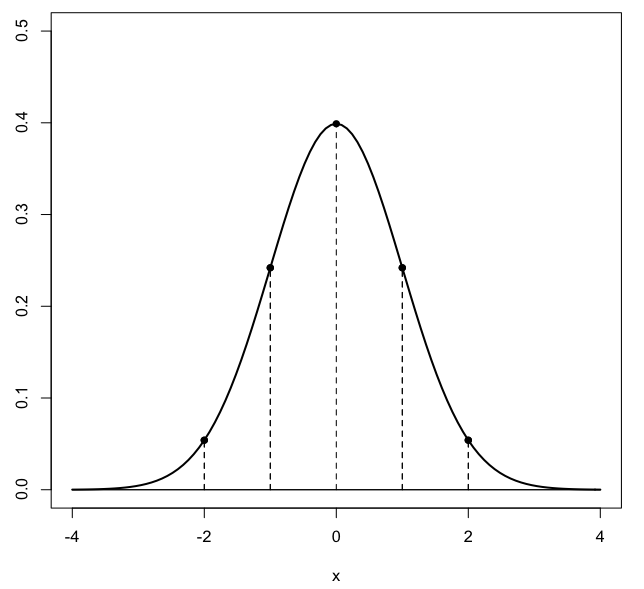
\includegraphics [scale=0.4] {gauss3.png} \end{center}

\title{Chain rule}
\date{}

\begin{document}
\maketitle
\Large

Here's a classic problem leading to the next idea.  Temperature in the atmosphere depends on the altitude, decreasing about $3$ degrees F for each $1000$ feet increase in altitude above sea level.
\[ T = T_0 - 3 h \]
\[ \frac{dT}{dh} = -3 \]
(In degrees F per thousand feet).

Suppose we're ascending a mountain road at a rate of $500$ feet per minute.
\[ \frac{dh}{dt} = 0.5 \]
(In thousands of feet per minute).

What is the rate of change of temperature with time?  It will turn out that
\[ \frac{dT}{dt} = \frac{dT}{dh} \cdot \frac{dh}{dt} = -3 \times 0.5 = -1.5 \]
(In degrees F per minute).

\subsection*{chain rule}
A compound function $f(g(x))$ means that we apply the function $g$ to the input $x$, then feed the output of that to the function $f$.  An example would be $\sin 2x$.

The chain rule says that if we have a compound function then
\[ \frac{d}{dx} \  f(g(x)) = f'(g(x)) \cdot g'(x) \]

If we break this down a bit we can write:
\[ t = g(x) \]
\[ y = f(t) = f(g(x)) \]
Then
\[ y' = f'(t) \cdot g'(x) = f'(g(x)) \cdot g'(x) \]

\begin{center} 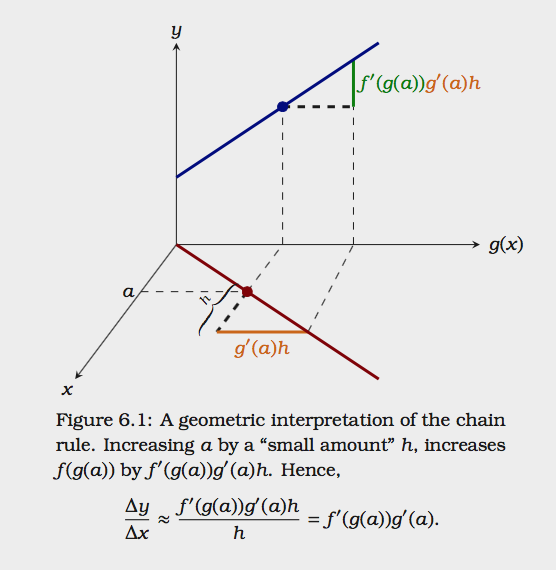
\includegraphics [scale=0.5] {chain_rule.png} \end{center}
For example
\[  \frac{d}{dx} \sqrt{1-x^2} = \frac{1}{2} \ \frac{1}{\sqrt{1-x^2}} \ (-2x) \]
\[ = - \frac{x}{\sqrt{1 - x^2}} \]
What we've done is to treat $1-x^2$ as one whole expression.  The factor of $-2x$ comes from the term $g'(x)$ in the chain rule.

We can do the same problem more slowly and clearly by substituting a new variable
\[ t = 1- x^2 \]
Take the derivative:
\[ \frac{dt}{dx} = -2x \]
Now rewrite the original $f(x)$ as $f(t)$:
\[ y = f(x) =  \sqrt{1-x^2}  \]
\[ y = f(t) = \sqrt{t} \]
\[ \frac{dy}{dt} = \frac{1}{2} \ \frac{1}{\sqrt{t}} \]

What we really wanted to know was $dy/dx$.  The chain rule says that
\[ \frac{dy}{dx} = \frac{dy}{dt} \ \frac{dt}{dx}  \]

(you can think of the factors of $dt$ as canceling, I won't tell anyone).
\[ =  \frac{1}{2} \ \frac{1}{\sqrt{t}} \ (-2x) \]
\[ = - \frac{x}{\sqrt{t}} \] 
\[ = - \frac{x}{\sqrt{1-x^2}} \]

\subsection*{common roots}

There are two common roots that we will run into in this book.  The first is the one given above where we might also have a constant $a^2$ and then
\[ \frac{d}{dx} \sqrt{a^2 - x^2} =  - x \ \frac{1}{\sqrt{a^2 - x^2}} \]
The power is $1/2$ which gives a factor of $1/2$ from the power rule.  The new power is then $1/2-1 = -1/2$, and we pick up a factor of $-2x$ from the chain rule.  The $2$'s cancel.

The second is
\[ \frac{d}{dx} (a^2 - x^2)^{3/2} = -3x \ \sqrt{a^2 - x^2} \]
The power is $3/2$ which gives a factor of $3/2$ from the power rule.  The new power is then $3/2-1 = 1/2$, and we pick up a factor of $-2x$ from the chain rule.  The $2$'s cancel.

We'll see both of these again a number of times.

\subsection*{proofs}
Proofs of the chain rule and the theorems in the next chapter can be found in almost any standard calculus text, but are really beyond the level of information we are targeting here.  The proof of the chain rule above basically depends on a property of limits.  If
\[ \lim_{x \rightarrow c} f(x) = L \]
\[ \lim_{x \rightarrow c} g(x) = M \]
then
\[ \lim_{x \rightarrow c} f(x) \ g(x) = LM \]
If you'd like to know more, there is an extensive chapter on Limits in the Addendum.


\end{document}